\chapter{COMPOSITE}

Pattern \underline{strutturale} (descrive la composizione di classi e oggetti), compone oggetti in strutture ad albero, adatto per tipi di dato ricorsivi.

Le classi client trattano questi oggetti in modo uniforme, indipendentemente dal fatto che si tratti di oggetti semplici o composti e non sanno (non 
devono sapere) se stanno interagendo con foglie o composti.

Sfrutta sia il meccanismo dell'ereditarietà e sia il meccanismo dell'object composition e delegation, il primo attraverso il fatto che un Composite è un Component, 
il secondo dove Composite è composto da tanti Component e delega operation() ai figli.

È facile aggiungere nuovi tipi di componenti, basta creare nuove sottoclassi di Leaf o di Composite, questi potranno essere usati immediatamente in strutture 
esistenti ma è difficile imporre dei vincoli sul tipo dei componenti.

Se un composto deve avere solo un certo tipo di figli, probabilmente il pattern non fa al caso nostro, questo pattern non può imporre vincoli statici, in 
quanto non possono essere controllati dal compilatore (type system) e quindi dovremmo effettuare controlli a runtime ed eventualmente, sollevare eccezioni (no good).

Un esempio di applicazione del pattern è il FileSystem, avremo la classe astratta FileSystemResource (il nostro Component), la sottoclasse FileSystemFile (Leaf) e 
FileSystemDirectory (Composite), che contiene al suo interno tanti oggetti di tipo FileSystemResource.

\section{Struttura}

\begin{figure}[H]
    \centering
    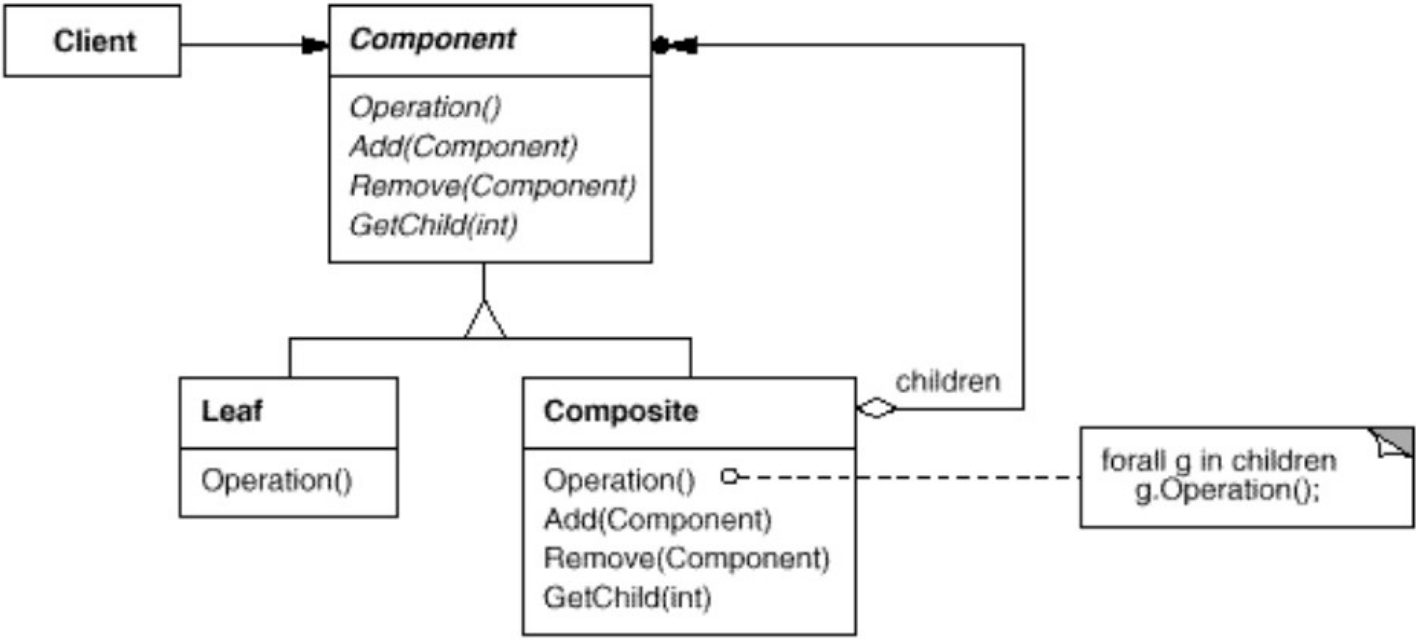
\includegraphics[width=0.5\linewidth]{../../immagini/composite/struttura_composite}
\end{figure}

\textbf{Component}
\begin{itemize}
    \item dichiara l’interfaccia comune a tutti gli oggetti della composizione;
    \item implementa il comportamento di default comune a tutte le sottoclassi, in questo caso operation();
    \item dichiara un’interfaccia per accedere a/e gestire i componenti figlio (add(), remove() e get());
    \item definisce un modo per accedere al componente padre (opzionale).
\end{itemize}

\textbf{Leaf}
\begin{itemize}
    \item rappresenta oggetti foglia della composizione;
    \item non ha figli;
    \item definisce il comportamento di default dell’interfaccia comune per gli oggetti primitivi della composizione.
\end{itemize} 

\textbf{Composite}
\begin{itemize}
    \item definisce il comportamento dell’interfaccia comune dei componenti con figli.
    \item memorizza i componenti figli;
    \item implementa le operazioni relativi alla gestione dei figli definite nell’interfaccia Component.
\end{itemize}

\textbf{Client} manipola gli oggetti della composizione attraverso l’interfaccia Component.
\medskip

Se la richiesta viene inviata ad una foglia, allora viene gestita direttamente, oppure se viene inoltrata ad un oggetto composto, allora viene inoltrata ai figli, 
facendo, eventualmente, delle operazioni prima e/o dopo l’inoltro.

\medskip
\textbf{N.B.}Le operazioni di gestione dei figli sono in Component, quindi Leaf li dovrebbe overridare sollevando un'eccezione oppure non facendo nulla.
\medskip

Per questo motivo abbiamo due versioni di questo pattern, una è quella che abbiamo visto ora, chiamata \textbf{design for uniformity}, e l'altra chiamata 
\textbf{design for tape safety} dove i metodi di gestione dei figli sono in Composite.

Nella prima i client, non sapendo se stanno trattando Leaf o Composite, potrebbero chiamare i metodi di gestione dei figli direttamente su Leaf, rischiando di 
ottenere errori a runtime.

Con l'altra versione il client non può chiamare operazioni per la gestione dei figli su Leaf, evitando così errori a runtime, può farlo solo Composite perdendo però 
uniformità.

Inolre il client dovrebbe avere un riferimento, di tipo statico, alla radice della struttura Composite, in caso contrario non potrebbe chiamare i metodi per 
gestire i figli.